\scanpage{52}
\mspage{\unsure{5}}
\[
\overline\psi_{G_1}:\zeta/\zeta_0=\pi_0^*\longrightarrow\uline{\operatorname{Hom}}(\pi_0,\pi_1)/\zeta_0
\]
déduit de $\psi_{G_1}$ par passage au quotient.
La condition à exprimer encore est

c) $\overline\psi_{G_1}$ est injective

Cette condition dépend effectivement de
$G_1$ à priori, puisque $\psi_{G_1}$ donc $\overline\psi_{G_1}$ en
dépend (de la manière explicitée plus
haut). Cette condition sur $G_1$ i.e. sur
\[
E_{\unsure{G}}\in\operatorname{Ob}\ \uline{\operatorname{Ext}}_{\mathrm{gr}}(\pi_0,\pi_1)
\]
\margin{(annulé\unsure{?})}

\figure{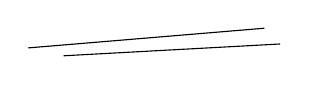
\begin{tikzpicture}\draw(0,0)--(3,.25);\draw(.45,-.1)--(3.2,.05);\end{tikzpicture}}

On veut exprimer maintenant
$N=DG$. Donc

 a) $N\supset DG$ i.e. $M'\ (=G/N)$ commutatif
\[
(\Longrightarrow\pi_0\text{ comm})
\]
Il faut exprimer ensuite que pour tout
ss-grpe \inserted{inv} $N_1\subset N$ tel que $G/N_1$ comm, on a
$N_1=N$. $G/N_1$ comm signifie que $G$ y
opère trivialt, cela implique qu'il opère
trivialt sur $N/N_1$ \inserted{et que celui-ci est comm}, or $G$ opère sur $N$
(ou $N/N_1$) via $M$, donc la condition est que
\deleted{$\unsure{N_1}$} $N/N_1$ est majoré par $\eta=N_{\unsure{\mathrm{comm}\,M|\mathrm{coinv}\,M}}$ \inserted{$=N/N_0$, i.e. $N_1\supset N_0$}.
Ceci dit dans l'extension \inserted{$G/N_0$} de $G/N=M'$ par
$\eta$, $G$ y opère, \inserted{en induisant l'id. sur les facteurs}, d'où un hom
\[
G\longrightarrow\uline{\operatorname{Hom}}(M',\eta)
\]
d'ailleurs nul sur $N$, d'où hom
\[
M'\longrightarrow\uline{\operatorname{Hom}}(M',\eta)
\]
\mspage{51}
